\documentclass[tikz]{standalone}

\usepackage{xcolor}
\definecolor{morange}{RGB}{255,127,14}
\definecolor{mblue}{RGB}{31,119,180}
\definecolor{mred}{RGB}{214,39,40}
\definecolor{mpurple}{RGB}{148,103,189}
\definecolor{mgreen}{RGB}{44,160,44}

\usepackage{mathtools}
\usepackage{amssymb}  
\usepackage{nicematrix} 

\usepackage{tikz}
\usetikzlibrary{fit,shapes.geometric}
\tikzset{highlight/.style={rectangle, draw=mblue, semithick, inner sep=1pt}}

\begin{document}

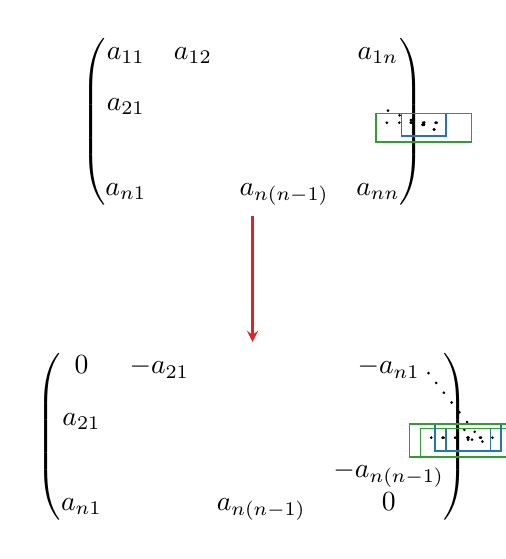
\begin{tikzpicture}

\node (matrix) {$
\begin{pNiceMatrix}[name=A]
     a_{11} & a_{12} & \Cdots & a_{1n}      \\
     a_{21} & \Ddots &        & \Vdots \\
     \Vdots & \Ddots & \Ddots & \Vdots \\
     a_{n1} & \Cdots & a_{n(n-1)}      & a_{nn} 
     \CodeAfter
     \tikz \node [highlight, fit=(2-1)(2-1), mblue] {};
     \tikz \node [highlight, fit=(4-1)(4-3), mgreen] {};
\end{pNiceMatrix}
$};

\node[below of=matrix, yshift=-3cm] (skew_sym_matrix) {$
\begin{pNiceMatrix}[name=B]
     0 & -a_{21} & \Cdots & -a_{n1}      \\
     a_{21} & \Ddots &        & \Vdots \\
     \Vdots & \Ddots & \Ddots & -a_{n(n-1)} \\
     a_{n1} & \Cdots & a_{n(n-1)}      & 0 
     \CodeAfter
     \tikz \node [highlight, fit=(2-1)(2-1), mblue] {};
     \tikz \node [highlight, fit=(4-1)(4-3), mgreen] {};
     \tikz \node [highlight, fit=(1-2)(1-2), mblue] {};
     \tikz \node [highlight, fit=(1-4)(3-4), mgreen] {};
\end{pNiceMatrix}
$};

\draw[-stealth, thick, rounded corners, mred] (matrix) -- (skew_sym_matrix);

\end{tikzpicture}
\end{document}

\end{document}